%!TEX root = paper.tex
%\vspace{-0.15in}

%\section{Analysis of State of Art}

\section{Privacy-preserving Energy Transactions}
\label{sec:petra}
%\textcolor{red}{There will be a figure here.}
\begin{figure*}[ht]
\centering
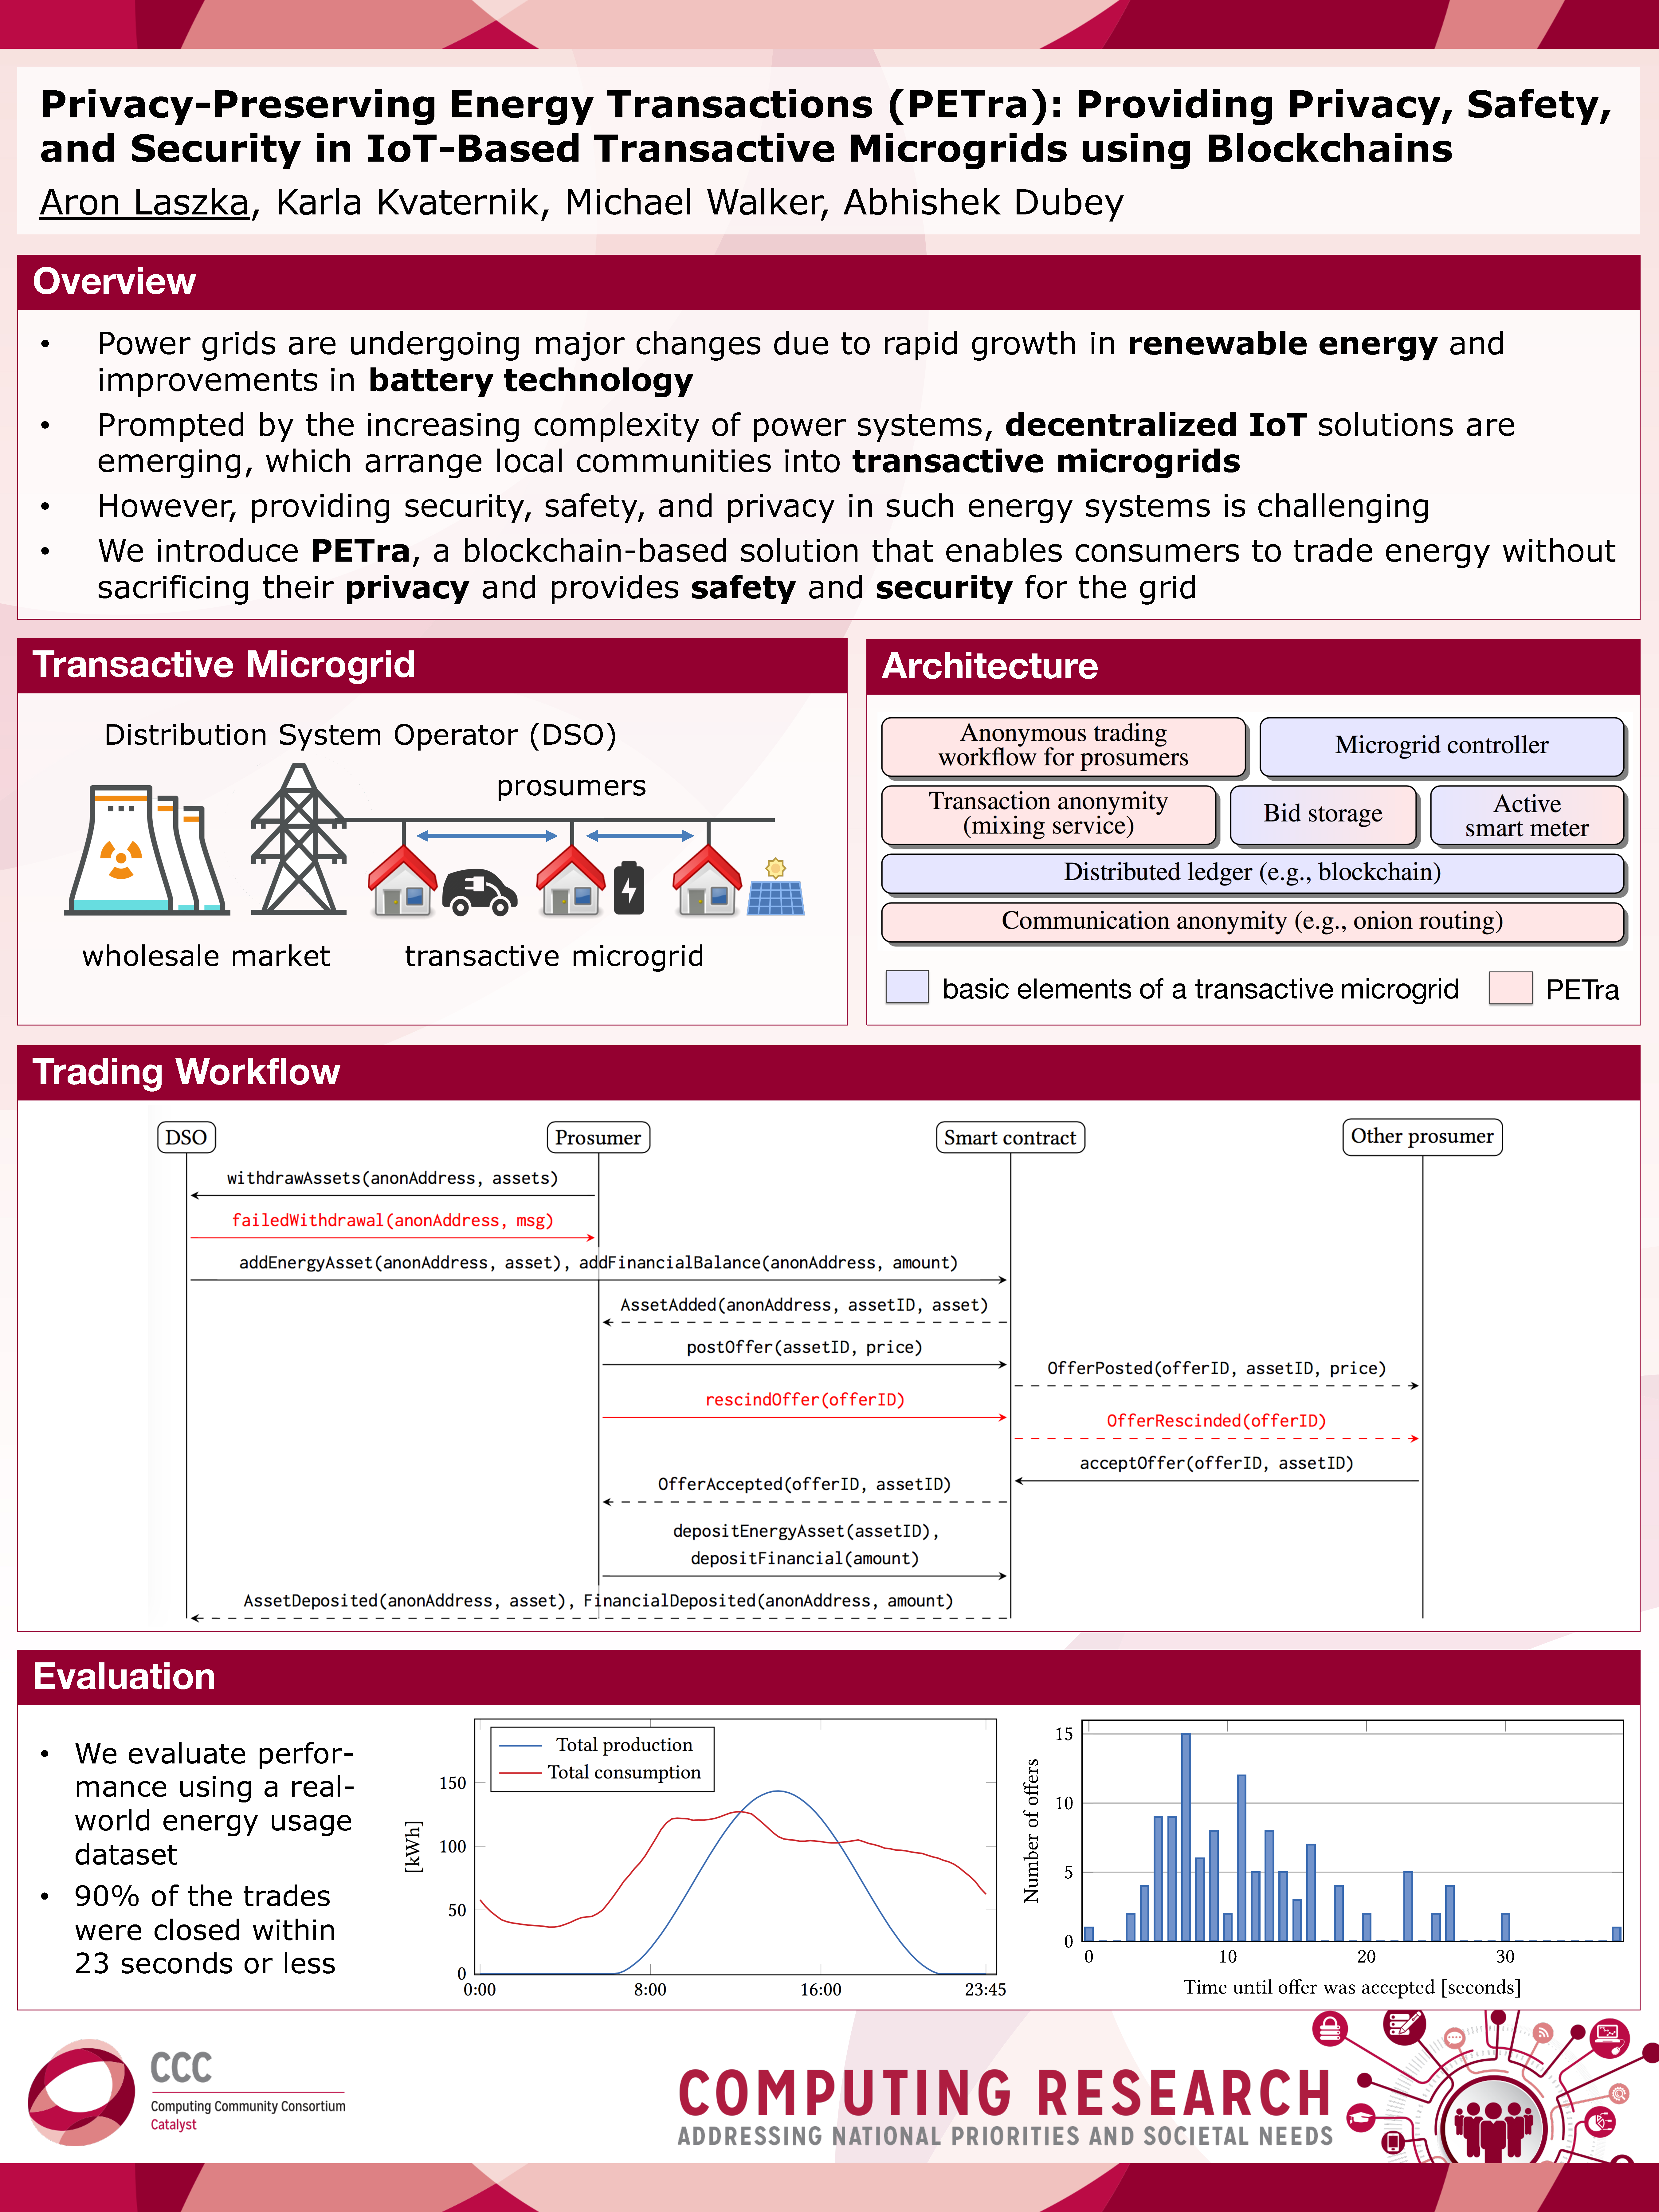
\includegraphics[width=\textwidth]{petra.pdf}
\caption{The sequence of activities in PETra. The red arrows show off-block chain communication and blue arrows show transactions on block-chain. Producers and consumers request the DSO to allocate the energy production and consumption assets to blockchain. The consumers receive asynchronous notification about offers from producers. Thereafter, they can finalize transaction. The energy transfer happens at a later time and is also recorded in the chain. Financial transactions are also done on the blockchain. These financial transactions are later tallied with the energy transactions.}\label{fig:petrasequence}
\end{figure*}

There is a systematic pattern emerging in the domain of Internet of Things which requires transactional capabilities. Examples include transactive ride-share systems \cite{yuan2016towards}, transactive health-care systems \cite{azaria2016medrec}, and transactive energy systems described earlier in this section. As shown in Figure \ref{fig:components}, there are three separate layers of this transaction. The first layer is the distributed ledger, which is responsible for keeping track of all log of all events of interest; in the energy domain these events are trades, energy transfer and financial transactions. In case of health care domain, the events record the time of access of the health care data. The data itself is not stored in the block-chain due to the size and privacy issues. Rather, the data is stored in the second layer, which can be implemented by either a cloud or a decentralized storage service like Storj\footnote{https://storj.io/}. The third layer is the IoT layer, which is responsible for sensing and control. This third layer is typically implemented using messaging middlewares like MQTT, DDS, etc. 

\definecolor{CustomBlue}{RGB}{88, 154, 214}
\definecolor{CustomOrange}{RGB}{238, 124, 33}

\begin{figure}
\centering
\resizebox {\columnwidth} {!} {
\centering
\begin{tikzpicture}[x=1.5cm, y=1.8cm, font=\small,
  Component/.style={fill=white, draw, align=center, rounded corners=0.1cm, drop shadow={shadow xshift=0.05cm, shadow yshift=-0.05cm, fill=black}},
  Connection/.style={<->, >=stealth, shorten <=0.15cm, shorten >=0.15cm, very thick, CustomOrange}]

\foreach \pos/\name in {0/pros1, 0.8/pros2, 1.6/pros3} {
  \node [Component] (\name) at (\pos - 4, \pos) {\texttt{IoT Device, geth}};
}

%\node [Component] (dso) at (-1, 2.6) {\texttt{IoT device, geth}};

\fill [fill=black!10] (90:1.5) -- (200:1.5) -- (340:1.5) -- (90:1.5);

\foreach \pos in {90, 200, 340} {
  \node [Component] at (\pos:1.5) {Ethereum\\miner (\texttt{geth})};
}

\node [Component, dotted] (contract) at (0, 0) {Smart contract\\(\texttt{Blockchain})};

\draw [Connection, bend left=0] (pros1) to (pros2);
\draw [Connection, bend left=0] (pros2) to (pros3);
\draw [Connection, bend left=-60] (pros3) to (pros1);

%\draw [Connection, CustomBlue, bend right=15] (dso) to (contract);
\draw [Connection, CustomBlue, bend right=0] (pros1) to (contract);
\draw [Connection, CustomBlue, bend right=0, , shorten <=0.5cm] (pros2) to (contract);
\draw [Connection, CustomBlue, bend right=0] (pros3) to (contract);

\node [Component, minimum width=10.25cm, minimum height=0.7cm] at (-1.39, -1.6) {Decentralized storage service};
\draw [Connection] (-3.2, -1.35) -- (-3.2, -0.32)  node [midway, right,black] {bulk data};
\draw [Connection, CustomBlue, ->] (0, -1.35) -- (0, -0.27)  node [midway, right, align=left, black, yshift={-0.1cm}] {meta\\[-0.2em]data};
\end{tikzpicture}
}
\vspace{-0.1in}
\caption{Components of IoT Blockchain pattern. Typically the IoT devices communicate with each other over a messaging middleware (red arrows). They also communicate with blockchain and smart contracts  (blue arrows) through clients, for example the Ethereum geth client. The miners are entities responsible for validating the events/transactions. %The distributed storage service is not shown in the figure.
}
\vspace{-0.1in}
\label{fig:components}
\end{figure}




The key aspect of this pattern is the tight integration of distributed  messaging patterns between actors and the blockchain-based communication network used for transferring transactional information. For example, in the transactive energy domain,  PETra, described in \cite{Laszka17}, involves the interactions between distribution system operator, prosumer, and a smart contract. The smart contract is  responsible for keeping track of the energy and financial assets enabling prosumers to post trade offers and exchange assets when another prosumer decides to accept.


The  algorithm of PETra uses quantised energy asset tokens\footnote{There are two kinds of energy tokens: Energy Production Asset and Energy Consumption Asset. Token attributes include power and time interval for which the token is valid.} that can represent the non-negative amount of power to be produced or consumed (for example, measured in watts),  the time interval in which energy is to be produced (or consumed) and the  last time interval in which energy is to be produced (or consumed) (Figure \ref{fig:petrasequence} describes the full sequence of activity). These assets are withdrawn and submitted to anonymized accounts on behalf of prosumers by the distribution system operator, which is also responsible for validating that the specific prosumer has the  energy capacity for feasible trades given the assets. Once the DSO posts the assets into the blockchain, prosumers can trade between themselves using these quantised assets and anonymized addresses, hiding their identity from each other. The DSO is also responsible for releasing and managing the transfer of currencies, which are represented by financial assets, which is  simply an unsigned integer value, denominated in a fiat currency. In this workflow, there are both on- and off-blockchain communications between DSO and prosumer. The off-blockchain communication is required to request the transfer of assets. On-blockchain communication occurs via filters that track the posting of assets. Similarly, prosumers also communicate which each other via blockchain to indicate when an offer has been posted and when a transaction has cleared. 

While all of the transactive IoT systems require communication and transactional anonymity there are domain-specific requirements and challenges that must be considered.  These characteristics and requirements guide us in the description of the anonymization architecture that we describe in the rest of this paper. Specifically, these characteristics are as follows: 
 (1) transactions in a microgrid must clear in bounded time and any errors must be detected\footnote{Energy trades that have an impact on real-time control (e.g., selling energy production for the near future) must be permanently recorded on the ledger \emph{in time} since grid control signals cannot be delayed.}, (2) typically, there is a dedicated communication channel available in a microgrid that connects the prosumers and the distribution system operator, (3) the set of participants in the network are fixed and known ahead of time. Thus, a discovery procedure is typically not required, and (4) even though all the transactions are anonymous there is still a need for maintaining associativity of properties like maximum generation capacity\footnote{To prevent destabilization of the grid, a producer should not be allowed to bid more than its maximum generation capacity.}, reputation scores to prosumers as they participate in trades to maximize the likelihood of success, while reducing the likelihood of jeopardizing the stability of the microgrid\footnote{A prosumer with low reputation score might have a history of not fulfilling the energy transfer obligations}. In the next two sections, we describe the mechanisms for implementing communication and transaction anonymity in this workflow.



% This section describes a basic system model of transactive IoT
% microgrids and formulates security, safety, and privacy requirements.
% A microgrid is a collection of prosumers (residential nodes) that are
% arranged within the same distribution feeder and support exchange of
% power between them. A prosumer node includes a smart
% inverter and a smart meter, which control the flow of power into and
% out of the prosumer. A microgrid also contains a set of nodes that are responsible for isolating faults on the feeder.  The
% \emph{Distribution System Operator} (DSO) operates %a set of
% switching nodes to control the connection of the microgrid to the rest
% of the distribution system. The DSO is responsible for regulating the
% net electric power into and out of the microgrid. Starting from this
% model, we next introduce the transactive microgrid model.

% \subsection{Transactive Microgrid System Model}
% \Abhishek{This is the perfect paragraph to define transactive
%   microgrid as a special application of IoT spread over a large
%   area. Perhaps we can find a citation that makes this point.}  We
% describe a basic system model of decentralized transactive IoT
% microgrids.  We discuss the following components: a distributed ledger
% for recording transactions, a bid storage service that facilitates
% finding trade partners, a microgrid controller for regulating the
% microgrid load, and smart meters for measuring the prosumers' energy
% production and consumption.


% \begin{figure}[h!]
% \center
% \begin{tikzpicture}[x=8cm, y=0.7cm, font=\small,
%   nodeStyle/.style={rounded corners=0.1cm, drop shadow={shadow xshift=0.05cm, shadow yshift=-0.05cm, fill=black}}
% ]
% \draw [nodeStyle, fill=red!10]  (0, 1.65) rectangle    (1, 2.25) node [midway, align=center] {Communication anonymity (e.g., onion routing)};

% \draw [nodeStyle, fill=blue!10] (0, 2.4) rectangle    (1, 3.0) node [midway, align=center] {Distributed ledger (e.g., blockchain)};

% \draw [nodeStyle, fill=red!10]  (0, 3.15) rectangle (0.45, 4.05) node [midway, align=center] {Transaction anonymity\\[-0.2em](mixing service)};
% \draw [nodeStyle, left color=blue!10, right color=red!10] (0.47, 3.15) rectangle (0.72, 4.05) node [midway, align=center] {Bid storage};
% \draw [nodeStyle, left color=blue!10, right color=red!10] (0.74, 3.15) rectangle (1, 4.05) node [midway, align=center] {Active\\[-0.2em]smart meter};

% \draw [nodeStyle, fill=red!10] (0, 4.2) rectangle (0.49, 5.1) node [midway, align=center] {Anonymous trading\\[-0.2em]workflow for prosumers};
% \draw [nodeStyle, fill=blue!10] (0.51, 4.2) rectangle (1, 5.1) node [midway, align=center] {Microgrid controller};
% \end{tikzpicture}
% \caption{Architecture of a decentralized transactive microgrid with \mbox{PETra}.}
% \label{fig:softwareArchitecture}
% \end{figure}

% Figure~\ref{fig:softwareArchitecture} shows a decentralized
% transactive microgrid with PETra.  
% In this figure, components marked in blue are basic elements of the decentralized transactive microgrid,
% while components marked in red are added (or extended) by PETra.

% \subsubsection{Distributed Ledger}
% Distributed ledger technologies, usually summarized under the term "blockchain" provide a distributed, decentrilized and highly fault tolerant database to facilitate secure transactions (messages) between all participants, and immutably store these transactions.  

% \subsubsection{Bid Storage Service}
% In large networks of prosumers it might make sense -for the sake of scalability- to offer platform services where bids and calls for trades can be published.

% \subsubsection{Microgrid Controller (Distribution System Operator)}
% The DSO includes a controller that regulates the total load on the microgrid and from the microgrid to the distribution system. The controller first predicts load in the
% microgrid based on (1) bids and asks in the bid storage and (2)
% outstanding energy trades in the ledger.  By combining this
% information with the prediction for the rest of the grid, the
% controller produces a control signal that specifies how much the
% microgrid load should be decreased or increased. Based on this
% signal, the controller then updates the price policy for the microgrid
% to influence energy production and consumption.  We also assume the
% presence of a secondary controller that balances voltage and frequency
% in the microgrid.

% \subsubsection{Smart Meters}
% To measure the prosumers' energy production and consumption, a smart
% meter must be deployed at each prosumer.  As with any blockchain-connected device, it needs to be tamper-resistant, in this case to prevent electricity theft. 

% \subsection{Requirements}
% We now discuss the security, safety, and privacy requirements that
% must be satisfied by a transactive energy IoT system.

% \subsubsection{Security}
% Security requirements ensure primarily that prosumers are billed
% correctly, but they also provide necessary prerequisite properties for
% safety.
% More specifically, they require that
% \begin{itemize}[noitemsep,topsep=-\parskip]
% \item prosumers are billed correctly based on the energy prices set by
%   the DSO, their energy trades, and their actual energy production and
%   consumption measured by the smart meters,
% \item prosumers or outside attackers cannot change microgrid
%   regulatory policies that are set by the DSO, 
% \item prosumers cannot back out of trades unilaterally, and they
%   cannot tamper with other prosumers' trading or bidding,
% \item financial and physical impact of compromised or faulty nodes is
%   limited, and nodes can be banned by the DSO. 
% \end{itemize}

% \subsubsection{Safety}
% A large gap between the aggregate production and consumption threatens the stability of not only the microgrid but also the main
% power grid.  Therefore, prosumers should not be able to trade large
% amounts of energy that they are unlikely to deliver.
% Specifically, we require that 
% \begin{itemize}[noitemsep,topsep=-\parskip]
% \item the net amount of energy sold (or bought) by a prosumer is upper
%   bounded (by a limit set by the DSO), where the net amount of
%   energy sold is the difference between the amount of energy sold and
%   bought by the prosumer, and the net amount of energy bought is
%   defined analogously. %,
% \Aron{If we have space, add back the safety requirement on the bid storage (and also add back the relevant parts of the description of the trading workflow and the ``analysis.''}
% %\item the energy bids and asks posted by a prosumer are limited in a similar way.
% \end{itemize}
% In practice, the DSO can set the limits based on the prosumers' production and consumption capacities.

% \subsubsection{Privacy} 
% Privacy requirements ensure that the prosumers' privacy is not
% compromised when they participate in energy trading.  We use
% non-transactive smart metering as a baseline, and we require that
% the transactive system does not leak any additional information
% compared to this baseline.  More specifically, we require that
% \begin{itemize}[noitemsep,topsep=-\parskip]
% \item the corresponding smart meter and DSO shall gain and retain as little information regarding the energy produced, consumed, bought and sold by a prosumer,
% \item only the prosumer may know which bids and asks it has posted,
%   and no one can know who traded energy with whom.
% \end{itemize}


